\chapter{Lec 11 - Model Selection II}

\maketitle

\section{Subset Selection}
In this section we consider some methods for selecting subsets of predictors. To perform best subset selection, we fit a separate least squares regression for each possible combination of the $p$ predictors. That is, we fit all $p$ models selection that contain exactly one predictor, all $p(p-1)/2$ models that contain
exactly two predictors, and so forth. We then look at all of the resulting models, with the goal of identifying the one that is best.\\\\
The problem of selecting the best model from among the $2^p$ possibilities
considered by best subset selection is not trivial. This is usually broken up
into two stages
\begin{center}
    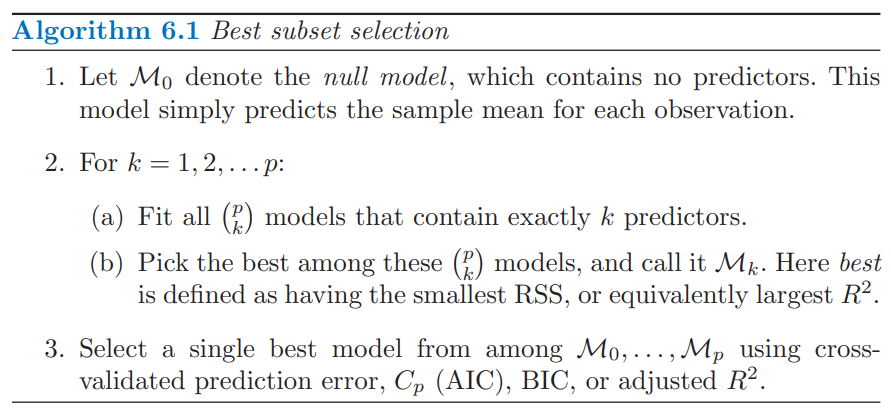
\includegraphics[scale=0.7]{images/best-subset.png}
\end{center}
In the algorithm above, Step 2 identifies the best model (on the training data)
for each subset size, in order to reduce the problem from one of $2^p$ possible models to one of $p + 1$ possible models. Now in order to select a single best model, we must simply choose among these $p + 1$ options. This task must be performed with care, because the RSS of these $p + 1$ models decreases monotonically, and the $R^2$ increases monotonically, as the number of features included in the models increases.\\\\
Therefore, if we use these statistics to select the best model, then we will
always end up with a model involving all of the variables. The problem is
that a low RSS or a high $R^2$ indicates a model with a low \textit{training error}, whereas we wish to choose a model that has a low \textit{test error}.
\\\\
Therefore, in Step 3, we use cross-validated prediction error, in order to select among $\mathcal{M}_0, \mathcal{M}_1, ..., \mathcal{M}_p$. While best subset selection is a simple and conceptually appealing approach, it suffers from computational limitations. The number of possible models that must be considered grows rapidly as $p$ increases.

\subsection{Stepwise Selection}
For computational reasons, best subset selection cannot be applied with
very large $p$. Best subset selection may also suffer from statistical problems when $p$ is large. The larger the search space, the higher the chance of finding models that look good on the training data, even though they might not have any predictive power on future data. Thus an enormous search space can lead to overfitting and high variance of the coefficient estimates. For both of these reasons, stepwise methods, which explore a far more restricted set of models, are attractive alternatives to best subset selection.
\paragraph{Forward Stepwise Selection.} Forward stepwise selection is a computationally efficient alternative to best subset selection. While the best subset selection procedure considers all $2^p$ possible models containing subsets of the $p$ predictors, forward stepwise considers a much smaller set of models. Forward stepwise selection begins with a model containing no predictors, and then adds predictors to the model, one-at-a-time, until all of the predictors are in the model. In particular, at each step the variable that gives the greatest \textit{additional} improvement to the fit is added to the model. More formally, the forward stepwise selection procedure is given in the following algorithm:
\begin{center}
    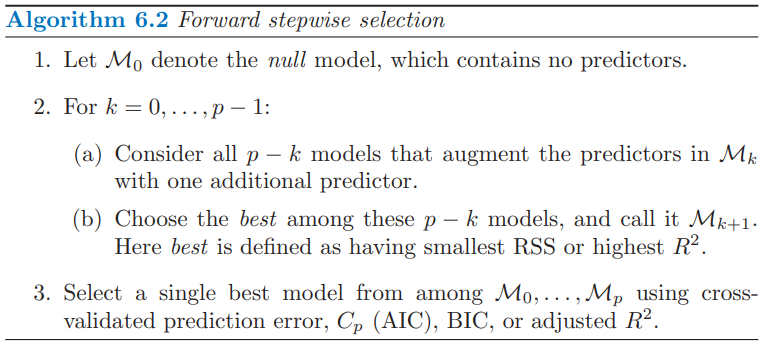
\includegraphics[scale=0.7]{images/forward stepwise.png}
\end{center}
Unlike best subset selection, which involved fitting $2^p$ models, forward
stepwise selection involves fitting one null model, along with $p - k$ models
in the $k$-th iteration, for $k = 0,...,p - 1$. This amounts to a total of $1 + \sum_{k=0}^{p-1} (p-k) = 1 + p(p+1)/2$ models.\\\\
In Step 2(b),  we must identify the best model from among those $p-k$ that augment $\mathcal{M}_k$ with one additional predictor. We can do this by simply choosing the model with the lowest RSS or the highest $R^2$. However, in Step 3, we must identify the best model among a set of models with different numbers of variables. This is more challenging, and
is discussed later.
\paragraph{Backward Stepwise Selection.} Like forward stepwise selection, backward stepwise selection provides an efficient alternative to best subset selection. However, unlike forward stepwise selection, it begins with the full least squares model containing all $p$ predictors, and then iteratively removes the least useful predictor, one-at-a-time.
\begin{center}
    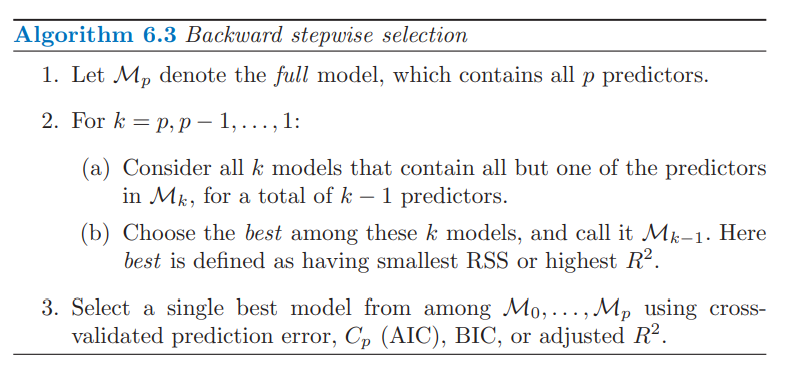
\includegraphics[scale=0.7]{images/backward stepwise.png}
\end{center}
Like forward stepwise selection, the backward selection approach searches
through only $1+p(p+ 1)/2$ models, and so can be applied in settings where
$p$ is too large to apply best subset selection. Also like forward stepwise
selection, backward stepwise selection is not guaranteed to yield the best
model containing a subset of the $p$ predictors.\\\\
Backward selection requires that the number of samples n is larger than
the number of variables $p$ (so that the full model can be fit). In contrast,
forward stepwise can be used even when $n<p$, and so is the only viable
subset method when $p$ is very large.
\paragraph{Hybrid Approaches.} The best subset, forward stepwise, and backward stepwise selection approaches generally give similar but not identical models. As another alternative, hybrid versions of forward and backward stepwise selection are available, in which variables are added to the model sequentially, in analogy to forward selection. However, after adding each new variable, the method may also remove any variables that no longer provide an improvement in the model fit. Such an approach attempts to more closely mimic best subset selection while retaining the computational advantages of forward and backward stepwise selection.

\subsection{Choosing the Optimal Model}
Best subset selection, forward selection, and backward selection result in the creation of a set of models, each of which contains a subset of the $p$ predictors. In order to implement these methods, we need a way to determine
which of these models is best. As we said previously, the model
containing all of the predictors will always have the smallest RSS and the
largest $R^2$, since these quantities are related to the training error. Instead, we wish to choose a model with a low test error.\\\\
In order to select the best model with respect to test error, we need to estimate this test error. There are two common approaches:
\begin{enumerate}
    \item We can indirectly estimate test error by making an adjustment to the training error to account for the bias due to overfitting.

    \item We can directly estimate the test error, using either a validation set approach or a cross-validation approach.
\end{enumerate}
MSE is generally an underestimate of the test MSE. (Recall that MSE = $RSS/n$.) This is because
when we fit a model to the training data using least squares, we specifically estimate the regression coefficients such that the training RSS (but not the test RSS) is as small as possible. Therefore, training set RSS and training set $R^2$ cannot be used to select from among a set of models with different numbers of variables.\\\\
However, a number of techniques for adjusting the training error for the model size are available. We now consider four such approaches: $C_p$, \textit{Akaike information criterion} (AIC), \textit{Bayesian information criterion} (BIC), and adjusted $R^2$.\\\\
For a fitted least squares model containing $d$ predictors, the $C_p$ estimate
of test MSE is computed using the equation
\[C_p = \frac{1}{n} (RSS + 2d \hat{\sigma}^2)\]
where $\hat{\sigma}^2$ is an estimate of the variance of the error  associated with each response measurement. Essentially, the $C_p$ statistic adds a penalty of $2d \hat{\sigma}^2$ to the training RSS in order to adjust for the fact that the training error tends to underestimate the test error. Clearly, the penalty increases as the number of predictors in the model increases; this is intended to adjust for the corresponding decrease in training RSS.\\\\
The AIC criterion is defined for a large class of models fit by maximum
likelihood. In the case of linear models with Gaussian errors, maximum
likelihood and least squares are the same thing. In this case AIC is given by
\[\text{AIC} = \frac{1}{n\hat{\sigma}^2}(\text{RSS} + 2d \hat{\sigma}^2)\]
where, for simplicity, we have omitted an additive constant.\\\\
BIC is derived from a Bayesian point of view, but ends up looking similar
to $C_p$ (and AIC) as well. For the least squares model with $d$ predictors, the BIC is, up to irrelevant constants, given by
\[\text{BIC} = \frac{1}{n} (\text{RSS} + log(n)d\hat{\sigma}^2)\]
Like $C_p$, the BIC will tend to take on a small value for a model with a
low test error, and so generally we select the model that has the lowest
BIC value. Notice that BIC replaces the $2d \hat{\sigma}^2$ used by $C_p$ with a $log(n)d\hat{\sigma}^2$ term, where $n$ is the number of observations. Since $log\, n > 2$ for any $n > 7$, the BIC statistic generally places a heavier penalty on models with many variables, and hence results in the selection of smaller models than $C_p$.\\\\
The adjusted $R^2$ statistic is another popular approach for selecting among
a set of models that contain different numbers of variables. For a least squares model with $d$ variables, the adjusted $R^2$ statistic is calculated as
\[\text{Adjusted } R^2 = 1 - \frac{\text{RSS} / (n - d - 1)}{\text{TSS}/(n-1)}\]
Unlike $C_p$, AIC, and BIC, for which a small value indicates a model with
a low test error, a large value of adjusted $R^2$ indicates a model with a
small test error. Maximizing the adjusted $R^2$ is equivalent to minimizing
$\frac{RSS}{n - d - 1}$. The intuition behind the adjusted $R^2$ is that once all of the correct variables have been included in the model, adding additional noise variables will lead to only a very small decrease in RSS. Since adding noise variables leads to an increase in d, such variables will lead to an increase in $\frac{RSS}{n - d - 1}$, and consequently a decrease in the adjusted $R^2$. Therefore, in theory, the model with the largest adjusted $R^2$ will have only correct variables and no noise variables.
\paragraph{Validation and Cross-Validation} 
As an alternative to the approaches just discussed, we can directly estimate the test error using the validation set and cross-validation methods. We can compute the validation set error or the cross-validation error for each model under consideration, and then select the model for which the resulting estimated test error is smallest. This procedure has an advantage relative to AIC, BIC, $C_p$, and adjusted $R_2$, in that it provides a direct estimate of the test error, and makes fewer assumptions about the true underlying model. It can also be used in a wider range of model selection tasks, even in cases where it is hard to pinpoint the model degrees of freedom (e.g. the number of predictors in the model) or hard to estimate the error variance $\sigma^2$. However, cross-validation is computationally heavier than the previous methods.

\section{Principal Components Regression}
The principal components regression (PCR) approach involves constructing the first $M$ principal components, $Z_1,...,Z_M$, and then using these components as the predictors in a linear regression model that is fit using least squares. The key idea is that often a small number of principal components suffice to explain most of the variability in the data, as well as the relationship with the response. In other words, we assume that the directions in which $X_1,...,X_p$ show the most variation are the directions that are associated with $Y$.\\\\
While this assumption is not guaranteed to be true, it often turns out to be a reasonable enough approximation to give good results. If the assumption underlying PCR holds, then fitting a least squares model to $Z_1,...,Z_M$ will lead to better results than fitting a least squares model to $X_1,...,X_p$, since most or all of the information in the data that relates to the response is contained in $Z_1,...,Z_M$, and by estimating only $M << p$ coefficients we can mitigate overfitting.\\\\
We note that even though PCR provides a simple way to perform regression using $M<p$ predictors, it is \textit{not} a feature selection method. This is because each of the $M$ principal components used in the regression is a linear combination of all $p$ of the original features. In PCR, the number of principal components, $M$, is typically chosen by cross-validation.
